\documentclass[crop,tikz]{standalone}
\usepackage{tikz}

\begin{document}

\usetikzlibrary{arrows,shapes}
\definecolor{yellow}{rgb}{1.0, 1.0, 0.45} % 255/255/115
\definecolor{dkyellow}{rgb}{0.9, 0.9, 0.0} % % 230/230/0

\definecolor{ltorange}{rgb}{1.0, 0.74, 0.41} % 255/188/105
\definecolor{orange}{rgb}{0.96, 0.50, 0.0} % 246/127/0

\definecolor{ltred}{rgb}{1.0, 0.25, 0.25} % 255/64/64
\definecolor{red}{rgb}{0.79, 0.00, 0.01} % 201/0/3

\definecolor{ltblue}{rgb}{0.2, 0.73, 1.0} % 51/187/255
\definecolor{blue}{rgb}{0.12, 0.43, 0.59} % 30/110/150

\definecolor{ltltgreen}{rgb}{0.7, 1.00, 0.7} % 96/204/14
\definecolor{ltgreen}{rgb}{0.37, 0.80, 0.05} % 96/204/14
\definecolor{green}{rgb}{0.23, 0.49, 0.03} % 59/125/8
  
\definecolor{dkslate}{rgb}{0.18, 0.21, 0.28} % 47/53/72
\definecolor{mdslate}{rgb}{0.45, 0.50, 0.68} % 114/127/173
\definecolor{ltslate}{rgb}{0.85, 0.88, 0.95} % 216/225/229


\tikzstyle{annotation} = [black, font={\bf}]
\tikzstyle{arrow} = [annotation, >=latex, ->, ultra thick]
\tikzstyle{image} = [anchor=south west,inner sep=0]


\begin{tikzpicture}

    \node[image] (image) at (0,0) {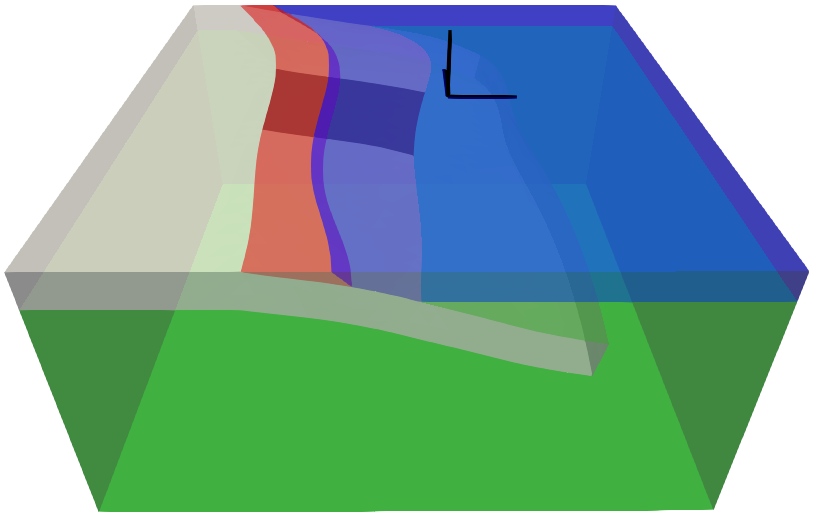
\includegraphics[width=5.5in]{subduction3d_geometry_patch}};
    \begin{scope}[x={(image.south east)},y={(image.north west)}]

      \node[anchor=west, annotation] (xneg) at (0.12,0.70) {Prescribed slip};
      \draw[arrow] (xneg) -- (0.35,0.77);
    \end{scope}

\end{tikzpicture}

\end{document}
